Based on the research outlined in the previous chapter, it was decided that an initial implementation of the proposed process would involve modelling the HRTF using principal components analysis to limit the number of variables in play to those those most significant components. Modifications to this reduced dataset would then be made based on simulated annealing search - with adjustments made where necessary. The efficacy of this implementation of this proposed approach has then been evaluated through listening tests conducted within a simple virtual reality environment. The metric for success is the same as the heuristic being used in the individualisation process - does the participant's ability to localise sound sources get better over time? If so, by how much?

\section{Algorithmic Design - unsure on current subsections}
\subsection{PCA}
For this implementation I elected to follow the model for PCA and PCW weight adjustment outlined by Josef Holzl\citep{Holzl2014a}. The core implementation would largely follow his formulation, as mapped out in the paper, with modifications where necessary. Having a method like this that allows for adaptation of the entire HRTF at once and helps to simplify the calculations that need to take place during the individualisation process, a convenience when a lot of the processing is taking place in real time. The input matrix structure that was decided upon during Holzl's investigation, [(Directions x Subjects)(Frequencies x 2)], was modified slightly to work for a single user to become: [Directions x (Frequencies x 2)]. In practical terms, an entry from the CIPIC HRIR database would be transformed into the frequency domain, resulting in an HRTF dataset in the form [Left/Right (2) x Azimuths (25) x Elevations (50) x Frequencies (101)]. This is then restructured into the above form, resulting in a structure [(Azimuths, Elevations (1250)) x (Frequencies, Left/Right (202))] in size. This structure is intuitive in terms of how the original values map to the new one, a quality that carries over even after the structure has been transformed with PCA. Performing PCA on this matrix effectively singles out the frequency bins that contain the most variance over all source directions. The resulting [PCW x PC] matrix is equivalent to [Directions x PCs] where the PCs are the frequency bins of greatest variance and the directions the PCWs. The benefit of this resulting structure is that it becomes very easy to modify the PCWs that relate to the position of a sound source. So for my implementation this means that it is simple to map the degree to which a user is able to locate a sound source to a relevant PCW within each PC. Because of this ability to match sound sources with principal component weights, coupled with the fact that PCW modifications were to be automated rather than performed manually, I chose not to model the resulting PCWs using spherical harmonics as Holzl did, further simplifying the individualisation process. 

The PCA model produced by this input matrix allows for around ninety percent of the variance in the to be described by 10 PCs, greatly limiting the number of variables that can be modified. This means that to adjust the perceived source of a sample the algorithm needs to only modify ten PCWs, one for each PCW that corresponds to that source position in each PC. 

\subsection{Simulated Annealing}
Core to simulated annealing (SA) search is that the degree of randomness, or the range of potential child states, is reduced as the current state gets closer to the goal state. In this implementation of the algorithm the value that is used to update the PCW is derived from user's localisation error, so the closer the user is to locating the sound source correctly, the smaller the change that is made to the PCW. It is worth noting that this implementation of this search method is effectively running 1250 individual searches in parallel, in order to find the optimal value for every individual source position so the process is unfortunately slow - this quality will be addressed in testing by limiting the number of possible source positions so that the effect of SA on individual source positions over time may be examined.

As mentioned above, modifying PCWs like this means that generating an individualised HRTF set would take at least 1250 seperate measurements, something that is almost as laborious as the standard measurement procedure. So to expedite the process, and to affect a greater amount of the HRTF with each modification, the PCWs for the eight source positions directly around the source being tested will also be modified by the same value, halved. This may mean that subsequent modifications partially overwrite previous ones, but it is preferable to expedite the process at least while data on the relationship between PCWs and localisation errors is so limited. 

Because there will be a not-insignificant amount of time betweeen each alteration made to a given PCW, the details of each alteration made are stored for future measurements from the same source position. This means that each time the algorithm begins to modify a set of PCWs, it first checks the existing database for previous adjustments. If extant, the previous error value, the modifier value for each PCW, and the change directions (whether the modifier was added to or subtracted from the weight within that PC) are all returned, and can inform this and subsequent changes. The direction of change is informed by whether or not this localisation attempt fared better than the previous one. If it did, then the change is made in the same direction. If it did not, some PCWs are adjusted the other way. In the event that a change is reversed and the next localisation attempt is better than the last, this system will ensure that the next change is made in the same direction(s). Given the aforementioned lack of research regarding the effect of the modification of different PCs on the perceived source of the sound, a decision had to be made regarding whether or not the update value was to be added to or subtracted from the current value of the PCW. The two options were to update every relevant PCW in the same direction, or to vary it. I decided on the latter, using different update directions in order to try and avoid situations where the algorithm might get caught in a loop, oscillating between two near-optimal states. The change was implemented using a process borrowed from genetic algorithms\citep{Whitley1994}, in which elements of a bit string are inverted based on a pseudorandom selection process, coupled with the SA's decreasing degrees of randomness. In this implementation a number of indexes in the update-directions matrix are selected at random, but the exact number that are selected is determined again by the degree of error in the user's localisation attempt. This solution should result in steadily more granular changes as the HRTF set becomes more well-suited to the user. 

\section{Implementation}
The project that has been produced to test this proposed method is formed of three parts: A VR test environment that manages the positions of the sound sources and processes the audio samples, passing data to another module for processing. This individualisation module forms the core of the implementation, as it handles the deconstruction, modification, and reconstruction of the HRTF data. This module is then tied to an in-memory key-value datastore that holds the starting HRTFs, intermediate results, and an archive of the changes made so far. In this test implementation the VR environment and individualisation module run on different machines. This was necessary for ease of development, but it is also an interesting idea for potential future implementations using a similar method, if such a system could be built to aggregate PCW/localisation error data, using it to train a model that takes that data and returns customised HRTFs. 

\begin{figure}
	\caption{HRTF Individualiser system diagram. }
	\centering{
		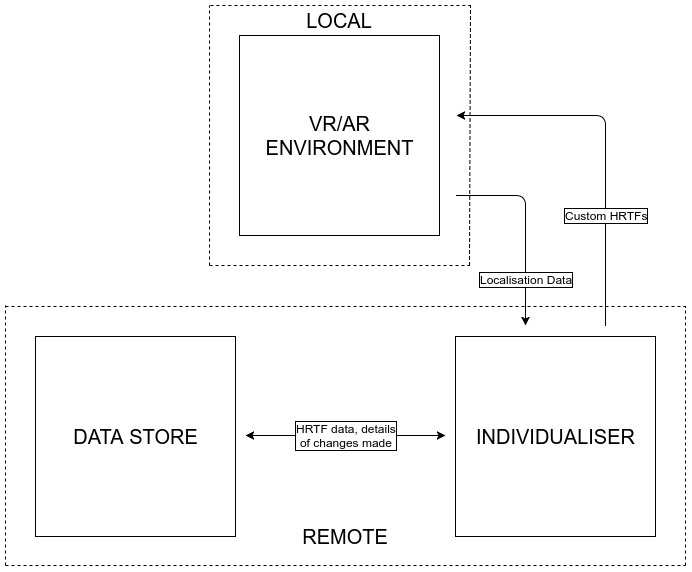
\includegraphics[scale=0.6]{individualiser_system_diagram}
	}
\end{figure}

\subsection{Technologies}
The bulk of the implementation is written in Python\citep{python lol}, making liberal use of the SciPy\citep{scipy and numpy} set of libraries to handle the majority of processing involved. Also in use is the simplejson\citep{simplejson} module, used to encode both HRTF data and logs extensively. To handle principal components analysis, the scikit-learn\citep{scikit learn} PCA class from the decomposition module was employed. Lastly, interfacing with the database was done using the lmdb module\citep{lmdb}. Symas' Lightning Memory-mapped Database \citep{lmdb db} was chosen both because it is a simple key-value datastore that doesn't require the kind of strictly defined strucure a relational database might, and because the entire contents of it can be loaded into memory when the program is started, making fetch and store operations comparatively rapid - useful when working in real-time. The test environment was produced using the Unity game engine \citep{•}, with the GoogleVR SDK \citep{•} and the Final Wireframe \citep{•} shader pack and run on a smartphone inside a Daydream\citep{•} viewer. The module and database are hosted on an Amazon Web Services (AWS) EC2 instance and communicate with the VR environment via TCP.

\subsection{Process}
Typically the individualisation process would run as follows, beginning with the user or participant in the VR space that is being used to generate the data. 

\begin{itemize}
\item The user faces a marker signifying the direction that relates to the 0, 0 angular coordinate for the CIPIC database.
\item The user is then played an audio cue that has been convolved with the corresponding HRIR from a source position that is generated at random but corresonds to a source position available in the database - in the case of CIPIC, this is anything from -45 degrees and up.
\item  Next, the user should point a reticle situated in the centre of their screen at where they think the sound originated from and issue some kind of confirmation. 
\item The perceived and actual sound source positions are then passed to the core module.
\item This information is then transformed into angular coordinates that match the way the CIPIC data is arranged, from which the update value is calculated like so:
\begin{itemize}
\item maths stuff
\end{itemize}
\item The current individualisation-in-progress HRTF is fetched from the database, along with a pre-prepared PCA model, and reformed into a [1250 x 202] input matrix. 
\item Next a matrix containing the mean value of each column in this matrix is subtracted from the input matrix and stored for later. 
\item The input matrix minus the mean is transformed using the PCA model, to produce the [1250 x 10] [PCWs x PCs] matrix. 
\item The database is then queried, to see if a modification has been made to this source position before, and the update value is used to adjust the PCWs according to the following conditions:
\begin{itemize}
\item If there is no data about previous adjustments, a set of ten boolean values are generated using Python's random module\citep{python random} to represent the adjustment direction for each principal component for that this weight (source position). 
\item Otherwise, if the data exists and the difference between the perceived and actual source positions in the most recent localisation attempt is greater than the previous one, a randomly chosen subset of the previously-used set of booleans have their values reversed and each PC is adjusted according to those directions. Otherwise, if the difference is lower, make the adjustment in the same direction. 
\end{itemize}
\item Information on the details of the adjustment made are then stored in the database, overwriting any previous data for changes made to that direction.
\item Once the PC matrix has been updated, the PCA transform is performed in reverse, and the column mean values are added back in.
\item Finally, this matrix is re-structured into the same format as the original HRTF matrix and stored in the database under the same key it was fetched from, archiving the previous iteration. 
\item This new, modified, HRTF is then used to process the next audio sample played to the user, and the process begins again. 
\end{itemize}

\subsection{Testing}
When it comes to analysing the efficacy of the approach, the tests will largely follow the above process with some small deviations. Because of the limited time available with each participant, I have run the process with the random source positions limited to a smaller subset of 8 key directions as opposed to the 1250 possible source positions if working with the full dataset. Limiting the source positions like this has allowed me to ensure that over the course of each test we are able to iterate over each source position several times, getting a better idea of how the PCWs change over time in relation to the error rate, and how localisation accuracy might change for a given direction over time. This limited set of source positions will be located in front of, behind, and to the left and right of the participant, as well as on the eight corners making up a cube around the participant like so: 

[DIAGRAM OF THE ARRANGEMENT]

The position of the sound source will change pseudorandomly, ensuring that the subject is tested from each source position the same number of times and that the same position isn't used twice in a row. For each position, the participant will be asked to face forward while the test sample, a one-second clip of pink noise, processed with the (semi)customised hrtf. The participants will have the option to play the sample again if they wish, and will be given ample time to try to locate the source position as accurately as they can. There will also be an on-screen indicator that displays when the participant is facing forward, allowing them to monitor their own head position.

During the tests, the individualisation module will automatically capture and all necessary for analysis. This includes the source location, perceived location, and resulting error value, as well as all of the primary PCWs both before and after they have been updated and what the direction of each update. All of this data is also timestamped, to make it easier to group data by test/participant. 

The main metric that I am interested in analysing after the tests is the error rate over time, in particular whether or not there is any decline in error rates as the test progresses. After that, I will also be looking to investigate whether or not there is any relationship between localisation errors, individual principal components, and update directions. Any potential relationship that exists there is interesting, because that information could be used to substantially enhance any future implementations of/updates to this individualisation process. There is enough variety in the captured data that answers to other questions may be investigated if time permits. 